\documentclass[12pt, draft, isbabel]{rureport}

\begin{document}

\maketitle

\tableofcontents

\listoffixmes

\clearpage

\section{Inngangur}\label{ch::inngangur}

Markmið verkefnisins er að hanna boltasamsetningu sem halda skal þremur stál stöngum saman. 
Við hönnun skal stærð, fjöldi og staðsetning bolta útfærð svo að samsetningin beri sem mest álag F, álagstilvik er sýnt á mynd \ref{fig::forsendur}. 
Athuga skal að myndin sýnir ekki heppilegt tilvik samsetningar. 

Nota skal 8.8 bolta ($S_y$ = 660 MPa og $S_{ut}$ = 830 MPa) og reikna með að efni í stöngum sé stál AISI 1020 HR ($S_y$ = 210 MPa og $S_{ut}$ = 380 MPa) eða sambærilegt. 
Reikna skal öll möguleg tilvik á að samsetningin eða stangirnar gefi sig. Samsetningin verður síðar prófuð og bera skal útkomu prófunarinnar saman við reiknuð gildi á mestu spennu. 
Ef útkoma prófana stangast á við reiknuð gildi skal gera grein fyrir ástæðum þess. 
Reikna má með því að undirstöðurnar eru staddar 1 cm frá enda stanga.

\begin{figure}[b]
	\centering
	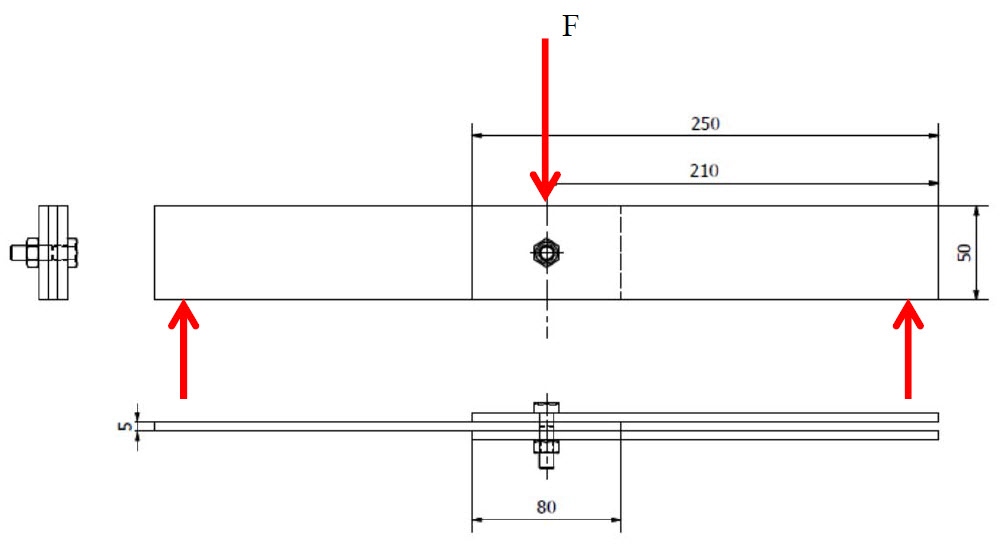
\includegraphics[width=1\textwidth]{forsendur}
	\caption{Álagstilvik verkefnisins}
	\label{fig::forsendur}
\end{figure}

\section{Reikningar}\label{ch::reikningar}

Við reikninga var miðað við eina plötu, \te þegar aðskilnaður flata hefur átt sér stað. 

Byrjað var á ytri greiningu samsetningarinnar. 
Þar sem ytra álag á samsetninguna er samhverft um miðju fæst að báðir undirstöðukraftarnir eru $R_{A} = R_{B} = F/2$, \sbr mynd \ref{fig::forsendur}. 
Við útreikninga var miðað við að mestu spennur sem boltinn eða efnið þyldi væru flotmörk, \te $n_y = 1$. 
Mesta beygjuspenna sem hver plata verður fyrir er í miðju samsetningarinnar, út frá því má finna mesta kraftinn sem hver plata þolir án þess að fara í flot.

\begin{equation}
  \sigma = {M c \over I} = {F l h \over 4I} 
  \Rightarrow F = {4 \sigma I \over l h}
  \label{eq::1}
\end{equation}

Í jöfnu \ref{eq::1} eru allar stærðir fastar nema flatartregðuvægið, I. 
Með því að lækka flatartregðuvægið mun mesti kraftur sem platan þolir fyrir flot minnka og því er ákveðið að bora ekki í miðja plötuna. 
Þessi kraftur, $F_{y,p}$, er því notaður sem lágmarksviðmið þegar stærð, staðsetning og fjöldi bolta er valin. 
Forsendur fyrir því að einhver tiltekin hönnunin virki er því að samsetningin má ekki fara í flot við minni kraft en $F_{y,p}$.

Flatartregðuvægið fyrir ferhyrnt þversnið er $I = {1 \over 12}bh^3$, því fæst að kraftur sem veldur því að samsetningin fari í flot í miðju:

\[
F_{y,p} 
= 
{
  4  \sigma_y I 
  \over 
  l h
}
= 
{
  \sigma_y b h^2 
  \over 
  3 l
} 
= 
{
  210 MPa \cdot 5 mm \cdot \left( 50 mm \right)^2 
  \over 
  3 \cdot 200mm
} 
= 4375N
\]

\subsection{Mismunandi tilvik semsetninga}

Plötur get vissulega farið í flot, en auk þess þarf að skoða þrjú önnur tilvik:

\begin{enumerate}
\item Beygjuspenna á yfirborði í þeirri línu, þvert á samsetninguna, sem götin eru boruð
\item Skerspenna sem boltar verða fyrir
\item Leguspenna sem verkar á efnið í götunum
\end{enumerate}

Til að minnka beygjuspennu á yfirborði er ákveðið að hafa götin sem næst lóðréttum brúnum samsetningarinnar.
Þannig er vægisarmurinn frá undirstöðunum styttur, sem minnkar beygjuspennuna \sbr jöfnu \ref{eq::1}. 
Við þetta hækkar skerspennan í boltum og leguspennan í götum efnisins. 
Til að koma til móts við þessa spennuhækkun er ákveðið að hafa götin sem fjærst láréttum brúnum samsetningarinnar, við það munu þær spennur lækka, \sbr jöfnu \ref{eq::2}\cite{shigleys}.

\begin{equation}
  F_n^{''} = {
    M r_n 
    \over 
    \displaystyle\sum_{i=1}^{k} r_i^2
  }
  \label{eq::2}
\end{equation}

$F_n^{''}$ er skerkraftur vegna vægis sem verkar á bolta n sem er í fjarlægð $r_n$ frá flatarmiðju boltanna og k er fjöldi bolta í samsetningunni. Tjakkurinn sem notaður verður við prófanir mun taka nær allt skerálagið frá kraftinum F, \sbr mynd \ref{fig::forsendur}, ef hönnunin er samhverf. Ef hönnunin er ekki samhverf myndast skerspenna í boltum vegna kraftsins F en hún er hverfandi miðað við skerkraft vegna vægis.

Því er hægt að nota jöfnu \ref{eq::2} til að finna skerspennu sem verkar á boltana og leguspennu sem verkar á efnið. 
Öll þrjú ofangreind tilvik voru tekin fyrir og skoðaðar þrjár samsetningar með tilliti til þeirra.
Í hverju tilfelli fyrir sig var krafturinn sem olli því að fyrrnefndar spennur færu í flot reiknaður.

\subsubsection{Fyrsta tilvik}

Í upphafi var einföld hönnun valin, \sbr mynd \ref{fig::2x6}. Vegna samhverfu um miðju er nóg að reikna aðeins fyrir annan boltann.

\begin{itemize}
\item Beygjuspenna á yfirborði við göt
  
  Jafna \ref{eq::1} er notuð við þetta en nú er flatartregðuvægið minna vegna holunnar. 
  Flatartregðuvægið er því $I = {1 \over 12}bh^3 - {1 \over 12}bd^3$. Því er sá kraftur sem veldur floti
  \[
  F = {4 \sigma I \over l h} 
  = {
    4 \cdot 210 MPa \cdot 
    \left(
      {
        1 \over 12
      } 
      \cdot 5 mm \cdot 
      \left(
        50mm
      \right)^3
      - 
      {
        1 \over 12
      } 
      5 mm \cdot 
      \left(
        6mm
      \right)^3
    \right) 
    \over 
    (160 mm + 12 mm) \cdot 50 mm
  } 
  = \underline{5080N}
  \] 

\item Skerspenna í bolta

  Jafna \ref{eq::2} er notuð til að finna skerkraftinn sem virkar á boltann

  \[
  F_1^{''} 
  = F_2^{''} 
  = {Mr_n \over 2r_n^2} 
  = 
  {
    {F \over 2}l \over 2 r_n
  } 
  \]

  Sá kraftur sem veldur því að skerspennan í boltanum nái flotspennu

  \[
  \sigma 
  = {F_1^{''} \over A_b} 
  \Rightarrow 
  F = 
  {
    4 S_{sy} A_b r_n \over l
  } 
  = {
    4 \cdot 
    {
      660MPa \over \sqrt{3}
    } 
    \cdot 
    {
      \pi \left(6mm\right)^2 \over 4
    } 
    \cdot 
    28 mm \over 200 mm
  } 
  = \underline{6030N}
  \]

\item Leguspenna í efni
  
  Sá kraftur sem verkar á leguna er skerkrafturinn sem verkar á bolta, því verður leguspennan
  
  \[
  \sigma 
  = {F_1^{''} \over bd} 
  \Rightarrow 
  F = {4 \sigma_{y} b d r_n \over l} 
  = 
  {
    4 \cdot 210 MPa \cdot 5 mm \cdot 6 mm \cdot 28 mm 
    \over 
    200mm
  } 
  = \underline{3528N}
  \]
\end{itemize}

Hér að ofan sést að sá kraftur sem veldur floti í legum efnisins er lægri en $F_{y,p}$ og því virkar þessu hönnun ekki miðað við þær forsendur sem við gáfum okkur.

\begin{figure}
  \centering
  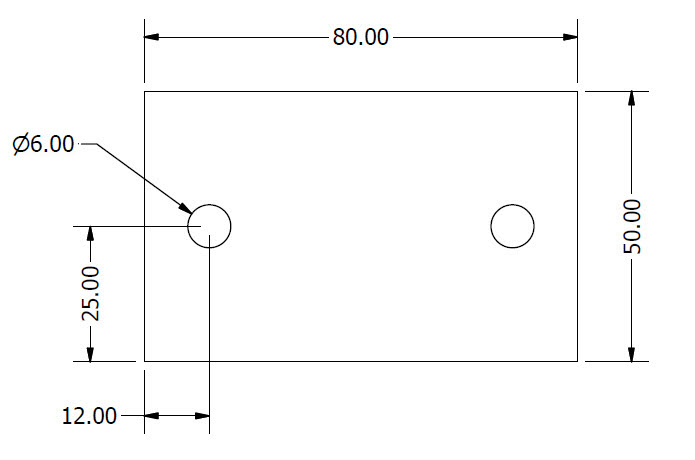
\includegraphics[width=0.5\textwidth]{2x6}
  \caption{Fyrsta reiknað tilvik}
  \label{fig::2x6}
\end{figure}

\subsubsection{Annað tilvik}

Þar sem fyrsta tilvik gekk ekki vegna leguspenna var athugað hvort 8 mm gat í stað 6 mm myndi standast forsendur okkar, \sbr mynd \ref{fig::2x8}. Vegna þess að aðeins ein breyting var gerð reiknast annað tilvikið líkt og það fyrsta.

\begin{itemize}
\item Beygjaspenna á yfirborði við göt
  
  \[
  F = {4 \sigma I \over l h} 
  = {
    4 \cdot 210 MPa \cdot 
    \left(
      {1 \over 12} 
      \cdot 5 mm \cdot 
      \left(
        50mm
      \right)^3 
      - 
      {1 \over 12} 5 mm \cdot 
      \left(
        8mm
      \right)^3
    \right) 
    \over 
    (160 mm + 12 mm) \cdot 50 mm
  } 
  = \underline{5066N}
  \] 
  
\item Skerspenna í bolta
  
  Á sama hátt og í fyrsta tilviki fæst sá kraftur sem veldur því að skerspennan í boltanum nái flotspennu
  
  \[
  \sigma = {F_1^{''} \over A_b} 
  \Rightarrow 
  F = {4 S_{sy} A_b r_n \over l} 
  = {4 \cdot {660MPa \over \sqrt{3}} 
    \cdot 
    {
      \pi 
      \left(
        8mm
      \right)^2 
      \over 
      4
    } 
    \cdot 28 mm \over 200 mm
  } 
  = \underline{10726N}
  \]
  
\item Leguspenna í efni
  
  Sá kraftur sem virkar á leguna er skerkrafturinn sem verkar á boltar, því verður leguspennan
  
  \[
  \sigma = {F_1^{''} \over bd} 
  \Rightarrow 
  F = {4 \sigma_{y} b d r_n \over l} 
  = {
    4 \cdot 210 MPa \cdot 5 mm \cdot 8 mm \cdot 28 mm 
    \over 
    200mm
  } 
  = \underline{4704N}
  \]

  \begin{figure}
    \centering
    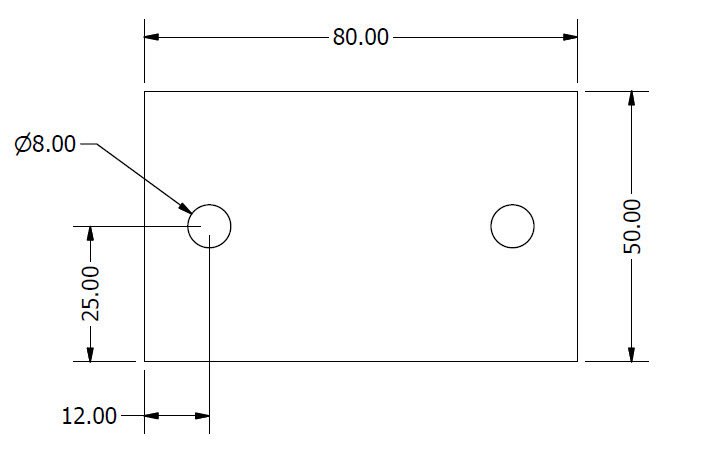
\includegraphics[width=0.5\textwidth]{2x8}
    \caption{Annað reiknað tilvik}
    \label{fig::2x8}
  \end{figure}

\end{itemize}

Eftir þessa breytingu fara leguspennur ekki í flot við kraft lægri en $F_{y,p}$ og því eru forsendurnar uppfylltar. 
Aftur á móti munar ekki miklu á kraftinum sem veldur floti í legum og $F_{y,p}$. Því er þriðja hönnunin gerð.

\subsubsection{Þriðja tilvik}

Aðeins flóknari hönnun er gerð í þriðja skiptið. 
Þá eru fjórir boltar notaðir í stað tveggja, \sbr mynd \ref{fig::4x6}. 
Vegna samhverfu dugir að reikna aðeins fyrir aðra hlið stykkisins og aðeins einn bolta þegar kemur að skerspennum og leguspennum.

\begin{itemize}
\item Beygjaspenna á yfirborði við göt
  
  Sá kraftur sem veldur floti fæst með jöfnu \ref{eq::1}. 
  Eina breyting frá fyrri tilvikum er flatartregðuvægið. 
  Í þessu tilfelli er flatartregðuvægið $I = {1 \over 12}bh^3 - 2\left({1 \over 12}bd^3\right)$. 
  Sá kraftur sem veldur floti á yfirborði plötu er því.
  
  \[
  F = \frac{4 \sigma I}{l h} 
  = 
  {
    4 \cdot 210 MPa \cdot 
    \left(
      {1 \over 12} \cdot 5 mm \cdot 
      \left(
        50mm
      \right)^3 
      - 2 \cdot 
      \left(
        {1 \over 12} \cdot 5 mm \cdot 
        \left(
          6mm
        \right)^3
      \right)
    \right) 
    \over 
    (160 mm + 12 mm) \cdot 50 mm
  } 
  = \underline{5070N}
  \] 
  
\item Skerspenna í bolta
  
  Vegna samhverfu bitans fæst sami kraftur í alla bolta og því nóg er að taka einungis fyrir einn bolta.
  
  \[
  F_1^{''} 
  = F_2^{''} 
  = F_3^{''} 
  = F_4^{''} 
  = {Mr_n \over 4r_n^2} 
  = {{F \over 2}l \over 4 r_n} 
  \]
  
  Í þessu tilviki er $r_n = \sqrt{(40mm - 12mm)^2 + (25mm - 13mm)^2} = 30.5 mm$. 
  Því fæst að sá kraftur sem veldur floti í boltum sé 
  \[
  \sigma = {F_1^{''} \over A_b} 
  \Rightarrow F 
  = {8 S_{sy} A_b r_n \over l} 
  = {8 \cdot {660MPa \over \sqrt{3}} \cdot 
    {
      \pi 
      \left(
        6mm
      \right)^2 
      \over 
      4
    } 
    \cdot 30.5 mm \over 200 mm
  } 
  = \underline{13144N}
  \]
  
  
\item Leguspenna í efni
  
  Líkt og áður þá er það skerkrafturinn sem verkar á boltana sem verkar á legu efnisins, því verður leguspenna í efninu
  
  \[
  \sigma = {F_1^{''} \over bd} 
  \Rightarrow F
  = {8 \sigma_{y} b d r_n \over l} 
  = {
    8 \cdot 210 MPa \cdot 5 mm \cdot 6 mm \cdot 30.5 mm 
    \over 
    200mm
  } 
  = \underline{7690N}
  \]

\end{itemize}

Við þessa hönnun fæst að sá kraftur sem veldur floti er töluvert hærri en viðmiðunarkrafturinn $F_{y,p}$ í öllum tilvikum. 
Því er þessi hönnun valin og smíðað eftir teikningu sem sjá má á mynd \ref{fig::smidamynd}.

Við smíði voru notaðir fjórir 8.8 M6x40 boltar. Gætt var að því að gengjur boltanna séu ekki staðsettar á samskeytum platnanna. Forspennukrafturinn var reiknaður sem $ 75\% $ af prufuálagi boltanna, \te 
$F_i = 0.75 \sigma_p A_t = 0.75 \cdot 600 MPa \cdot 20.1 mm^2 = 9045N$. Gengjurnar voru smurðar við herslu boltanna, því er hersluvægið sem þarf til að ná forspennukraftinum 

\[
T = K F_i d = 0.18 \cdot 9045N \cdot 6mm = 9.8 Nm
\]

Við semsetningu var því hert 10 Nm með hjálp herslumælis.

\begin{figure}
  \centering
  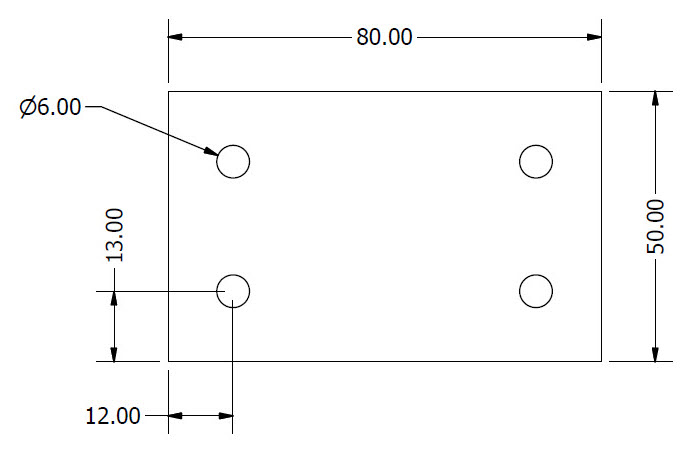
\includegraphics[width=0.5\textwidth]{4x6}
  \caption{Þriðja reiknað tilvik}
  \label{fig::4x6}
\end{figure}

\begin{figure}
	\centering
	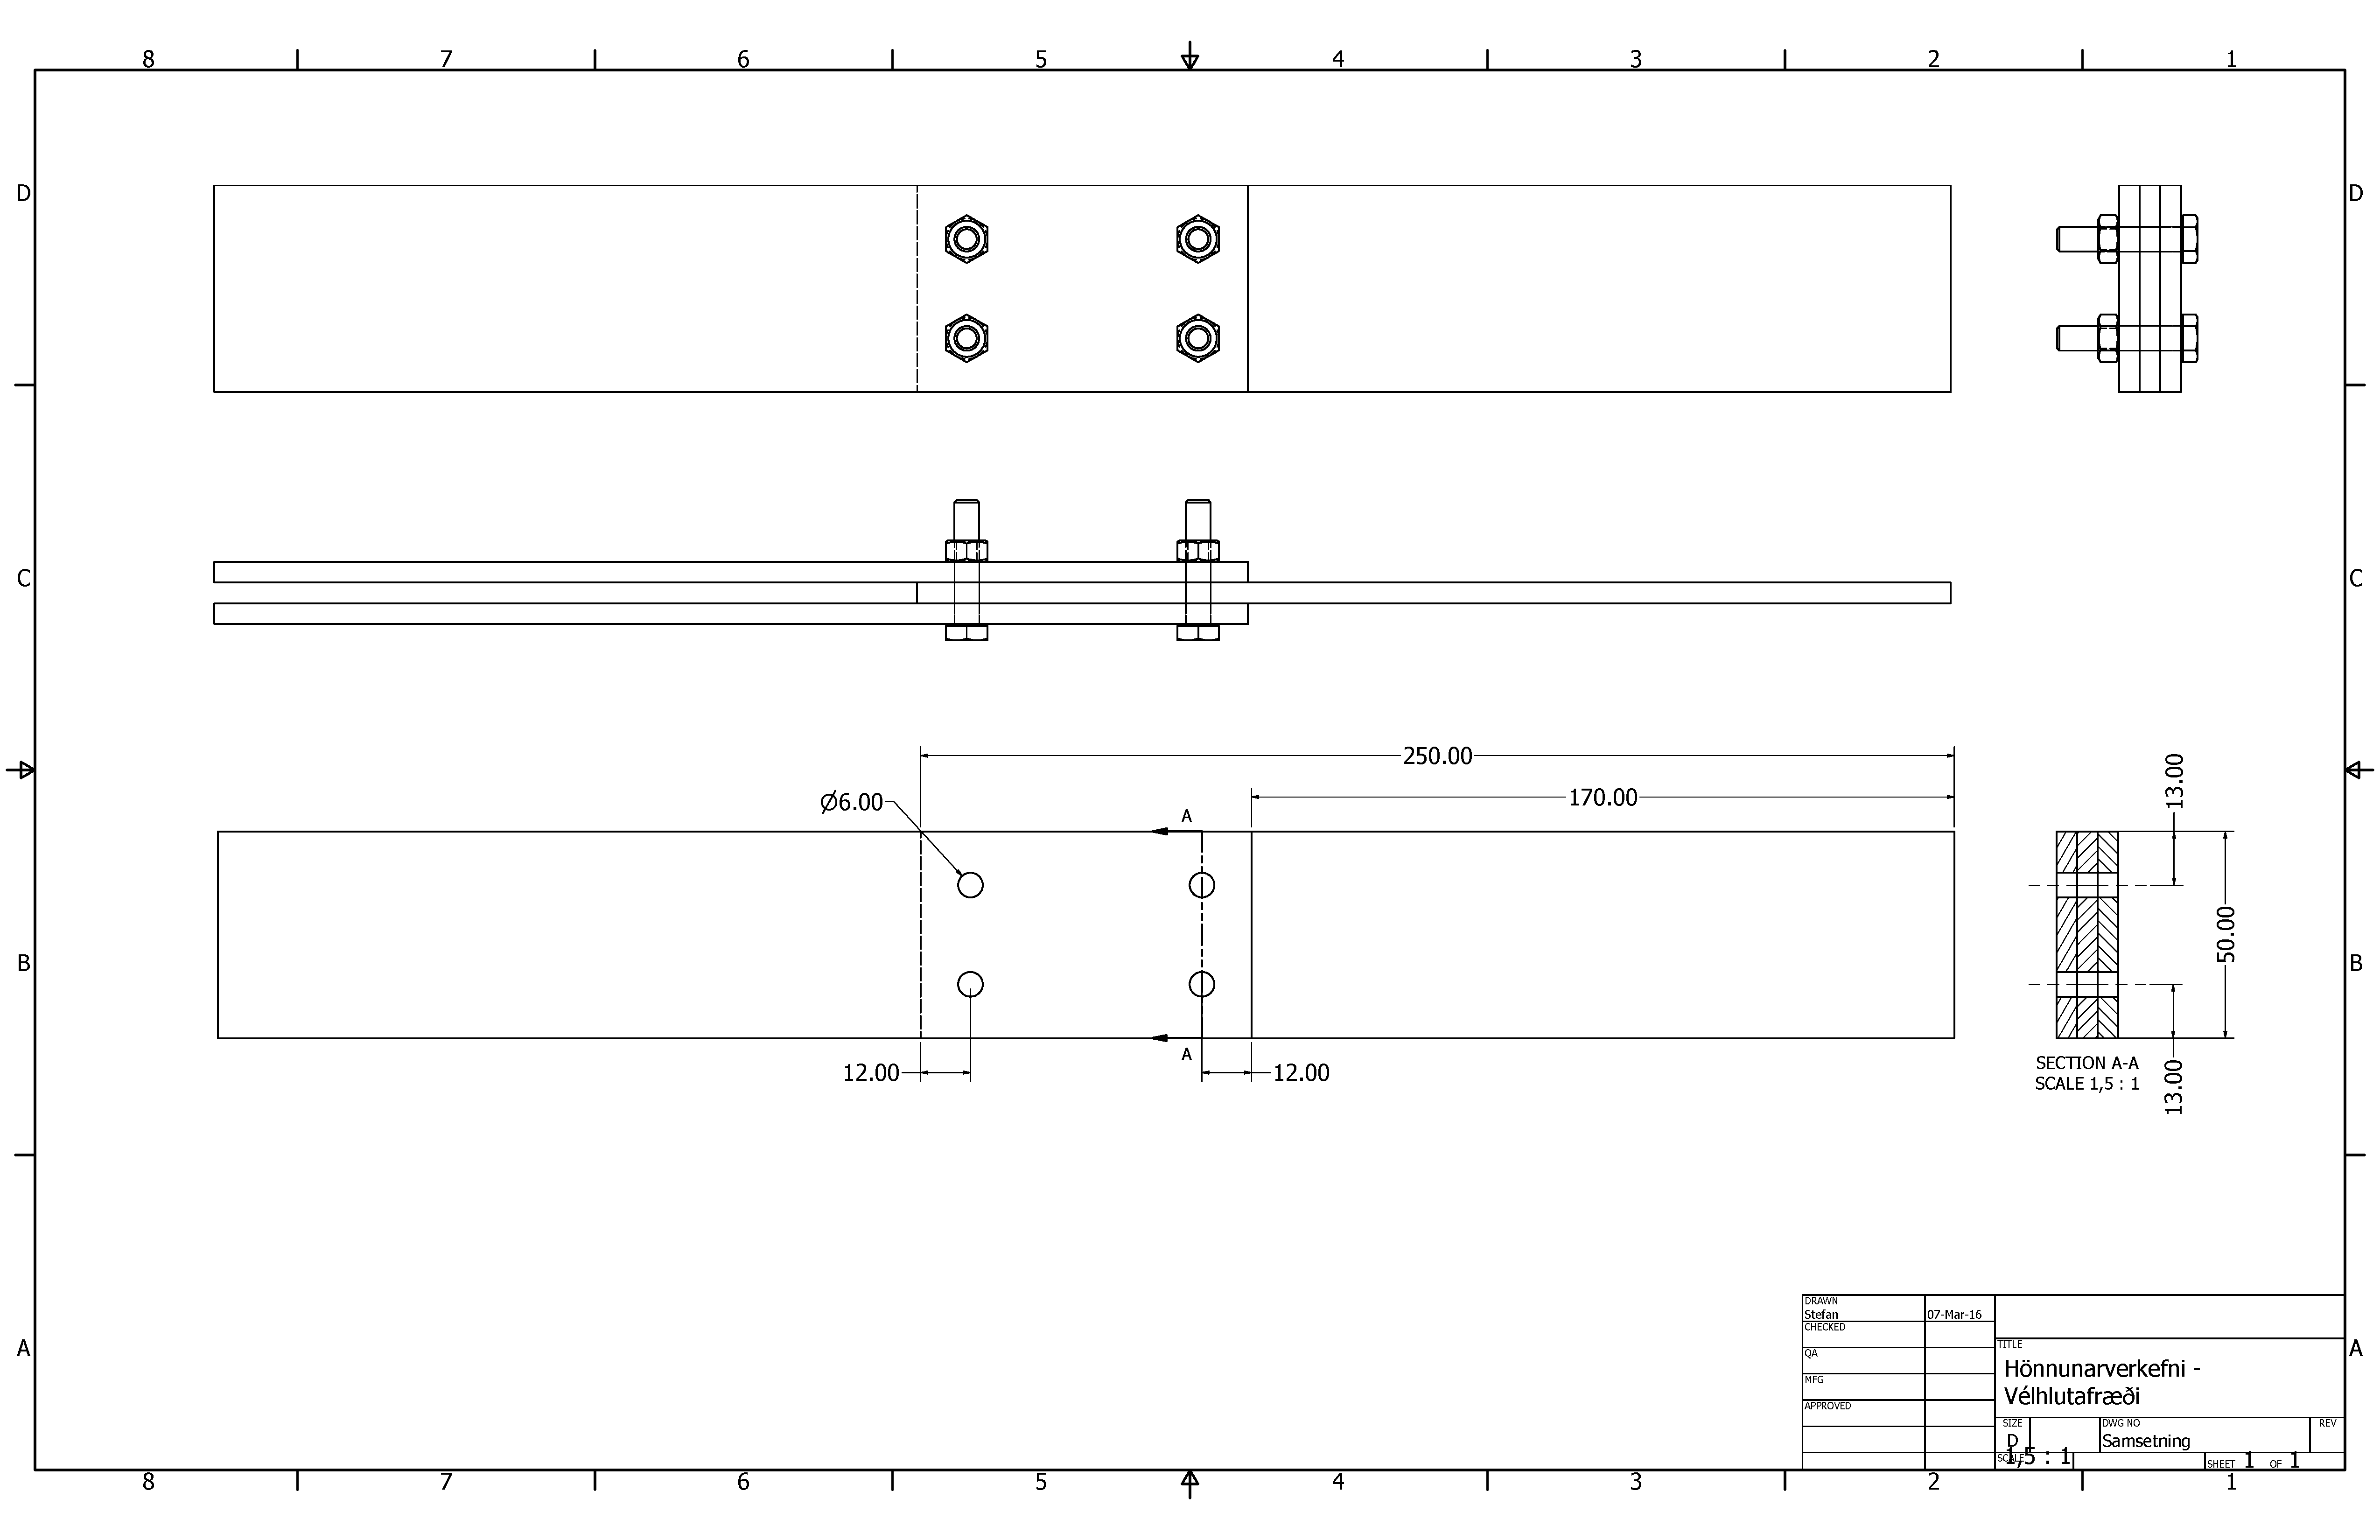
\includegraphics[width=1.4\linewidth, angle = 90]{Samsetning}
	\caption{Málsett smíðateikning sem smíðað var eftir}
	\label{fig::smidamynd}
\end{figure}


\section{Niðurstöður}
\label{sec:nidurstodur}

Samkvæmt útreikningum okkar hefðu plöturnar gefið sig á undan boltunum eða við $4375 N$, \sbr kafla \ref{ch::reikningar}.
Boltarnir hefðu átt að þola allt að \fxnote{álag sem boltar þola} álag.

\begin{figure}[h]
  \centering
  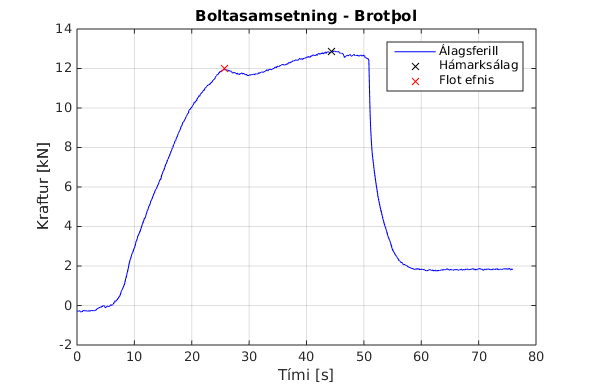
\includegraphics[width=\linewidth]{alag}
  \caption{Álagsferill í þolprófun}
  \label{fig:alag}
\end{figure}

Þar sem útreikningar okkar miðast við eina plötu, \te eftir að aðskilnaður hefur átt sér stað, er þetta ekki alveg rétt.
Ef reiknað væri með öllum plötunum, þ.e.~áður en aðskilnaður hefur átt sér stað, myndi flatartregðuvægið þrefaldast, sem passar nokkuð vel við þau gildi sem komu fram í prófunum.
Eins og sjá má á mynd \ref{fig:alag} kemst efnið í flot við \(12 kN \approx 4375 N \cdot 3 = 13.13 kN\) sem stenst nokkuð vel.
Skekkjan á því er þá \(100\% - {12 \over 13.13} = 8.61\% \)

\clearpage

\begin{figure}
  \centering
  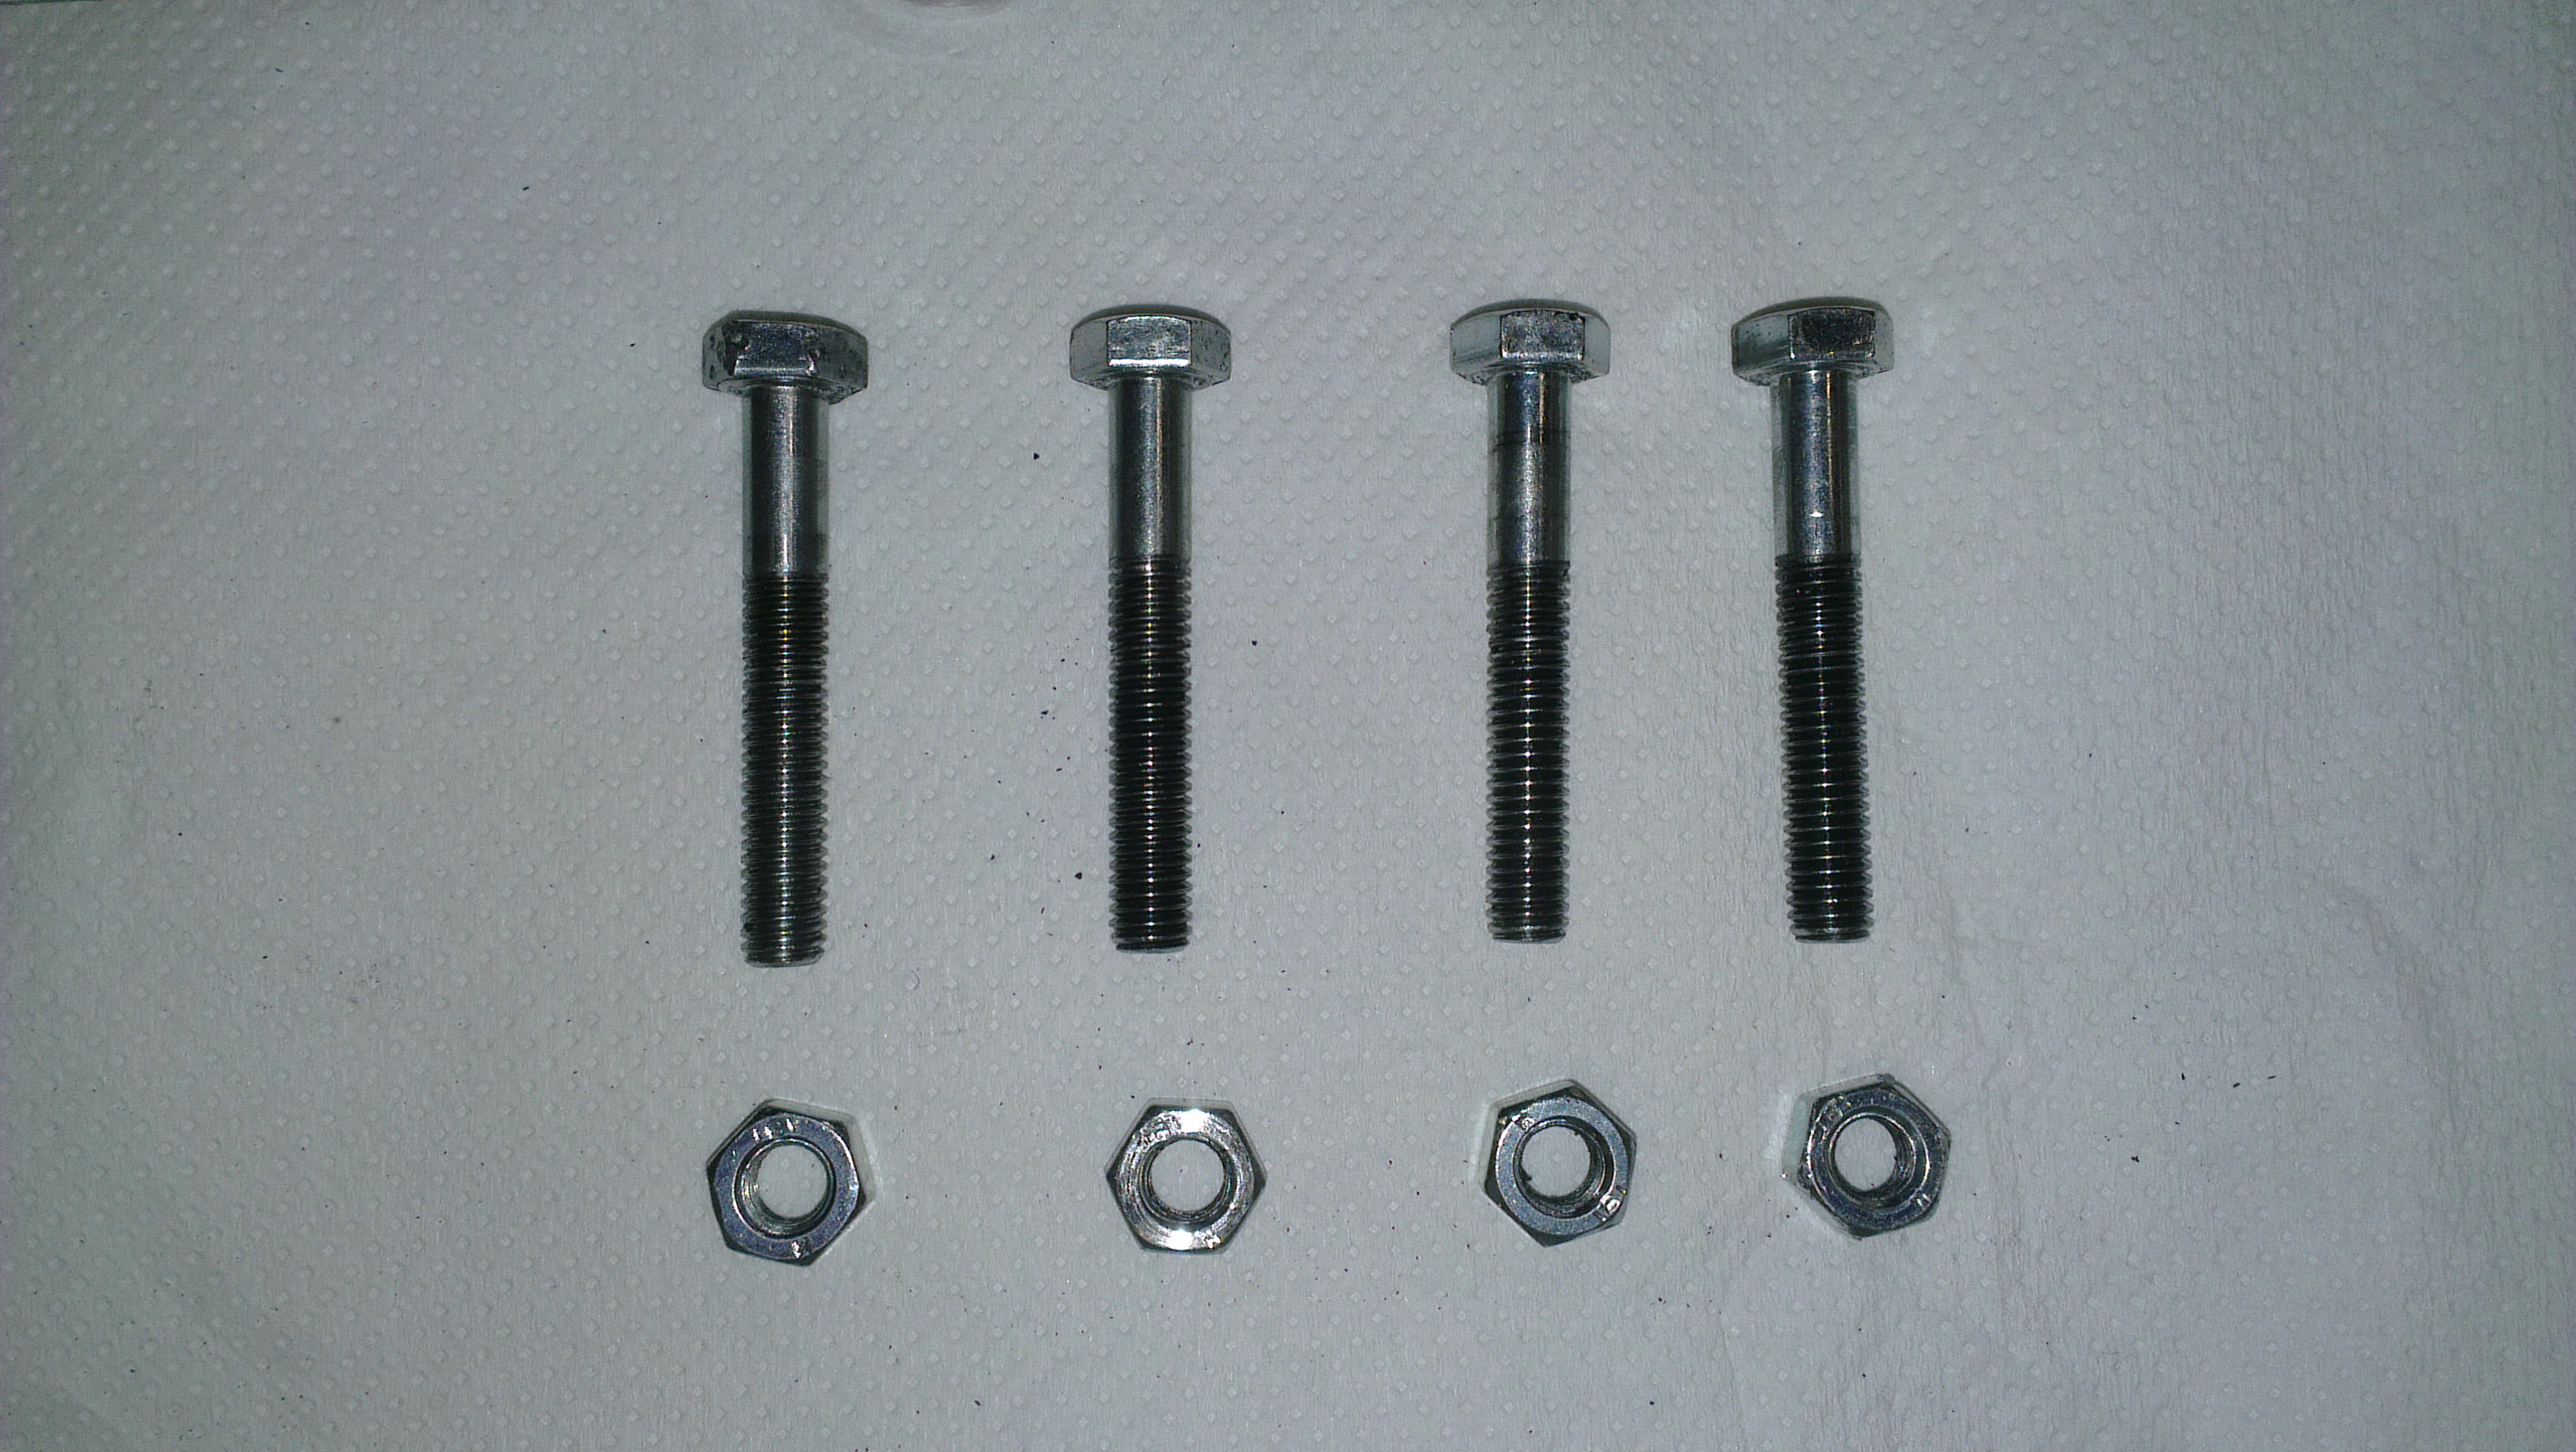
\includegraphics[width=\linewidth]{boltar}
  \caption{Boltar eftir prófun}
  \label{fig:boltar}
\end{figure}

\begin{figure}
  \centering
  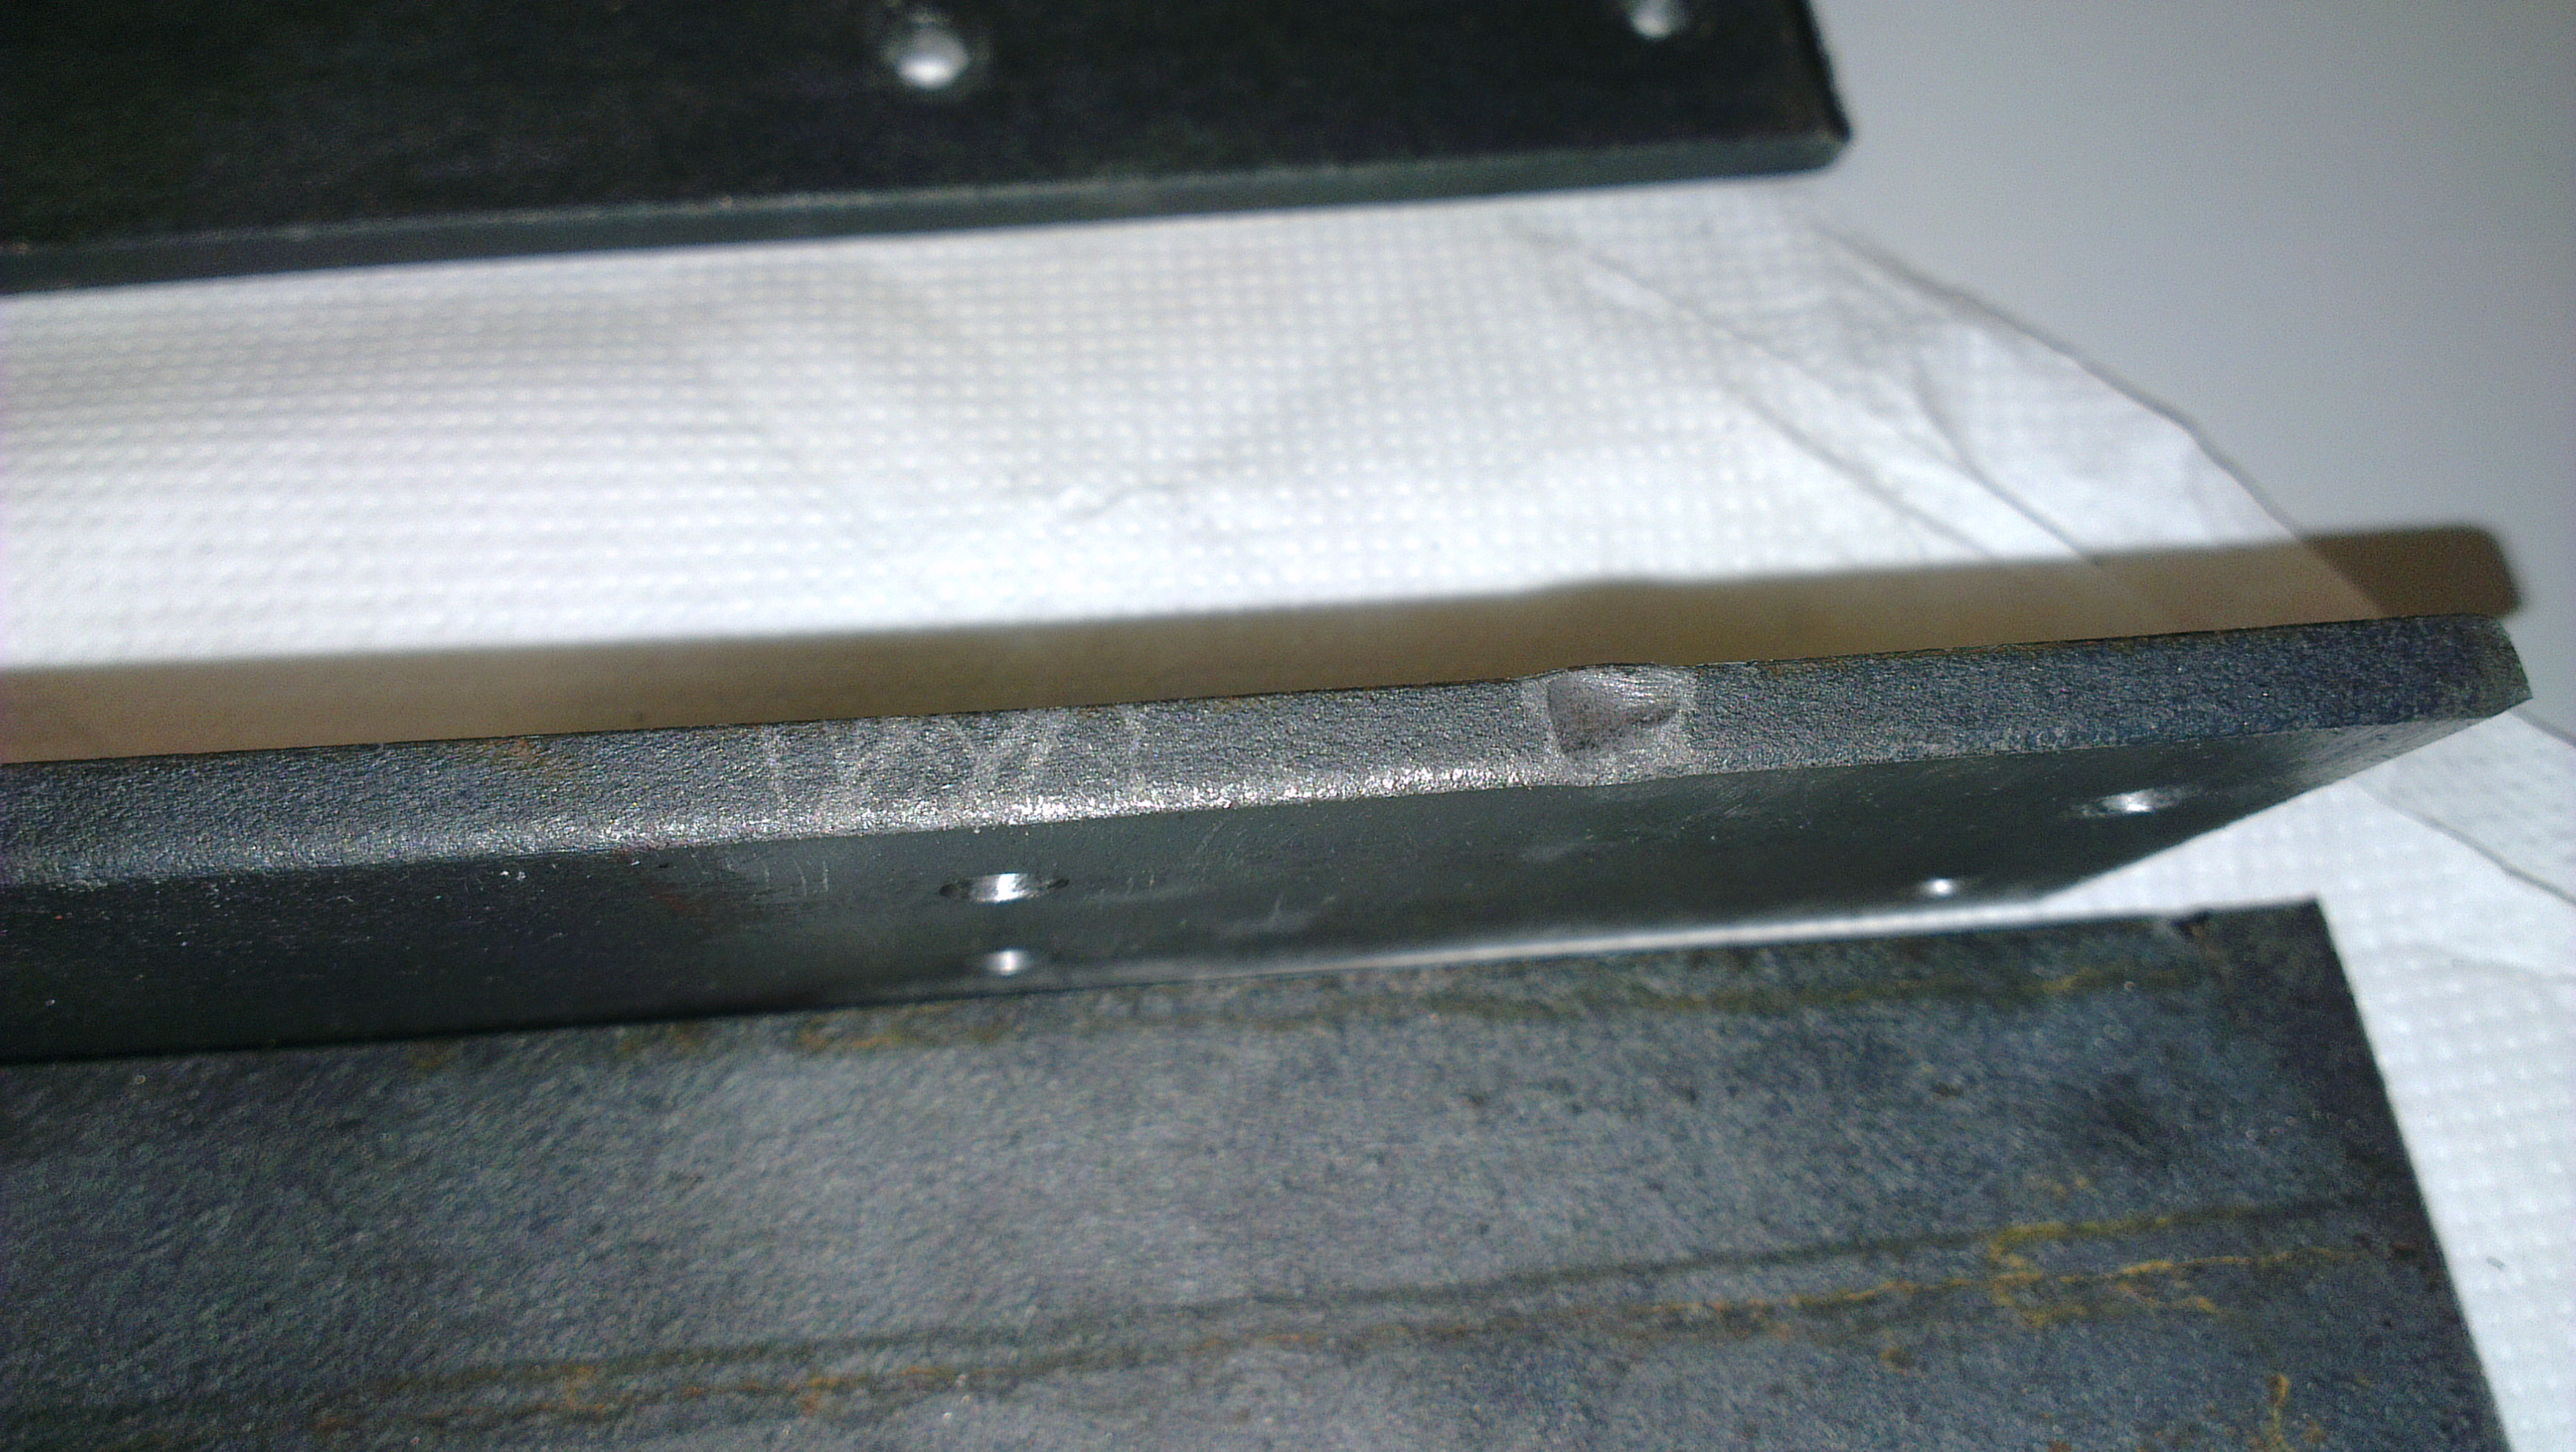
\includegraphics[width=\linewidth]{hak}
  \caption{Hak sem myndaðist í einni stöng við prófun}
  \label{fig:hak}
\end{figure}

\begin{figure}
  \centering
  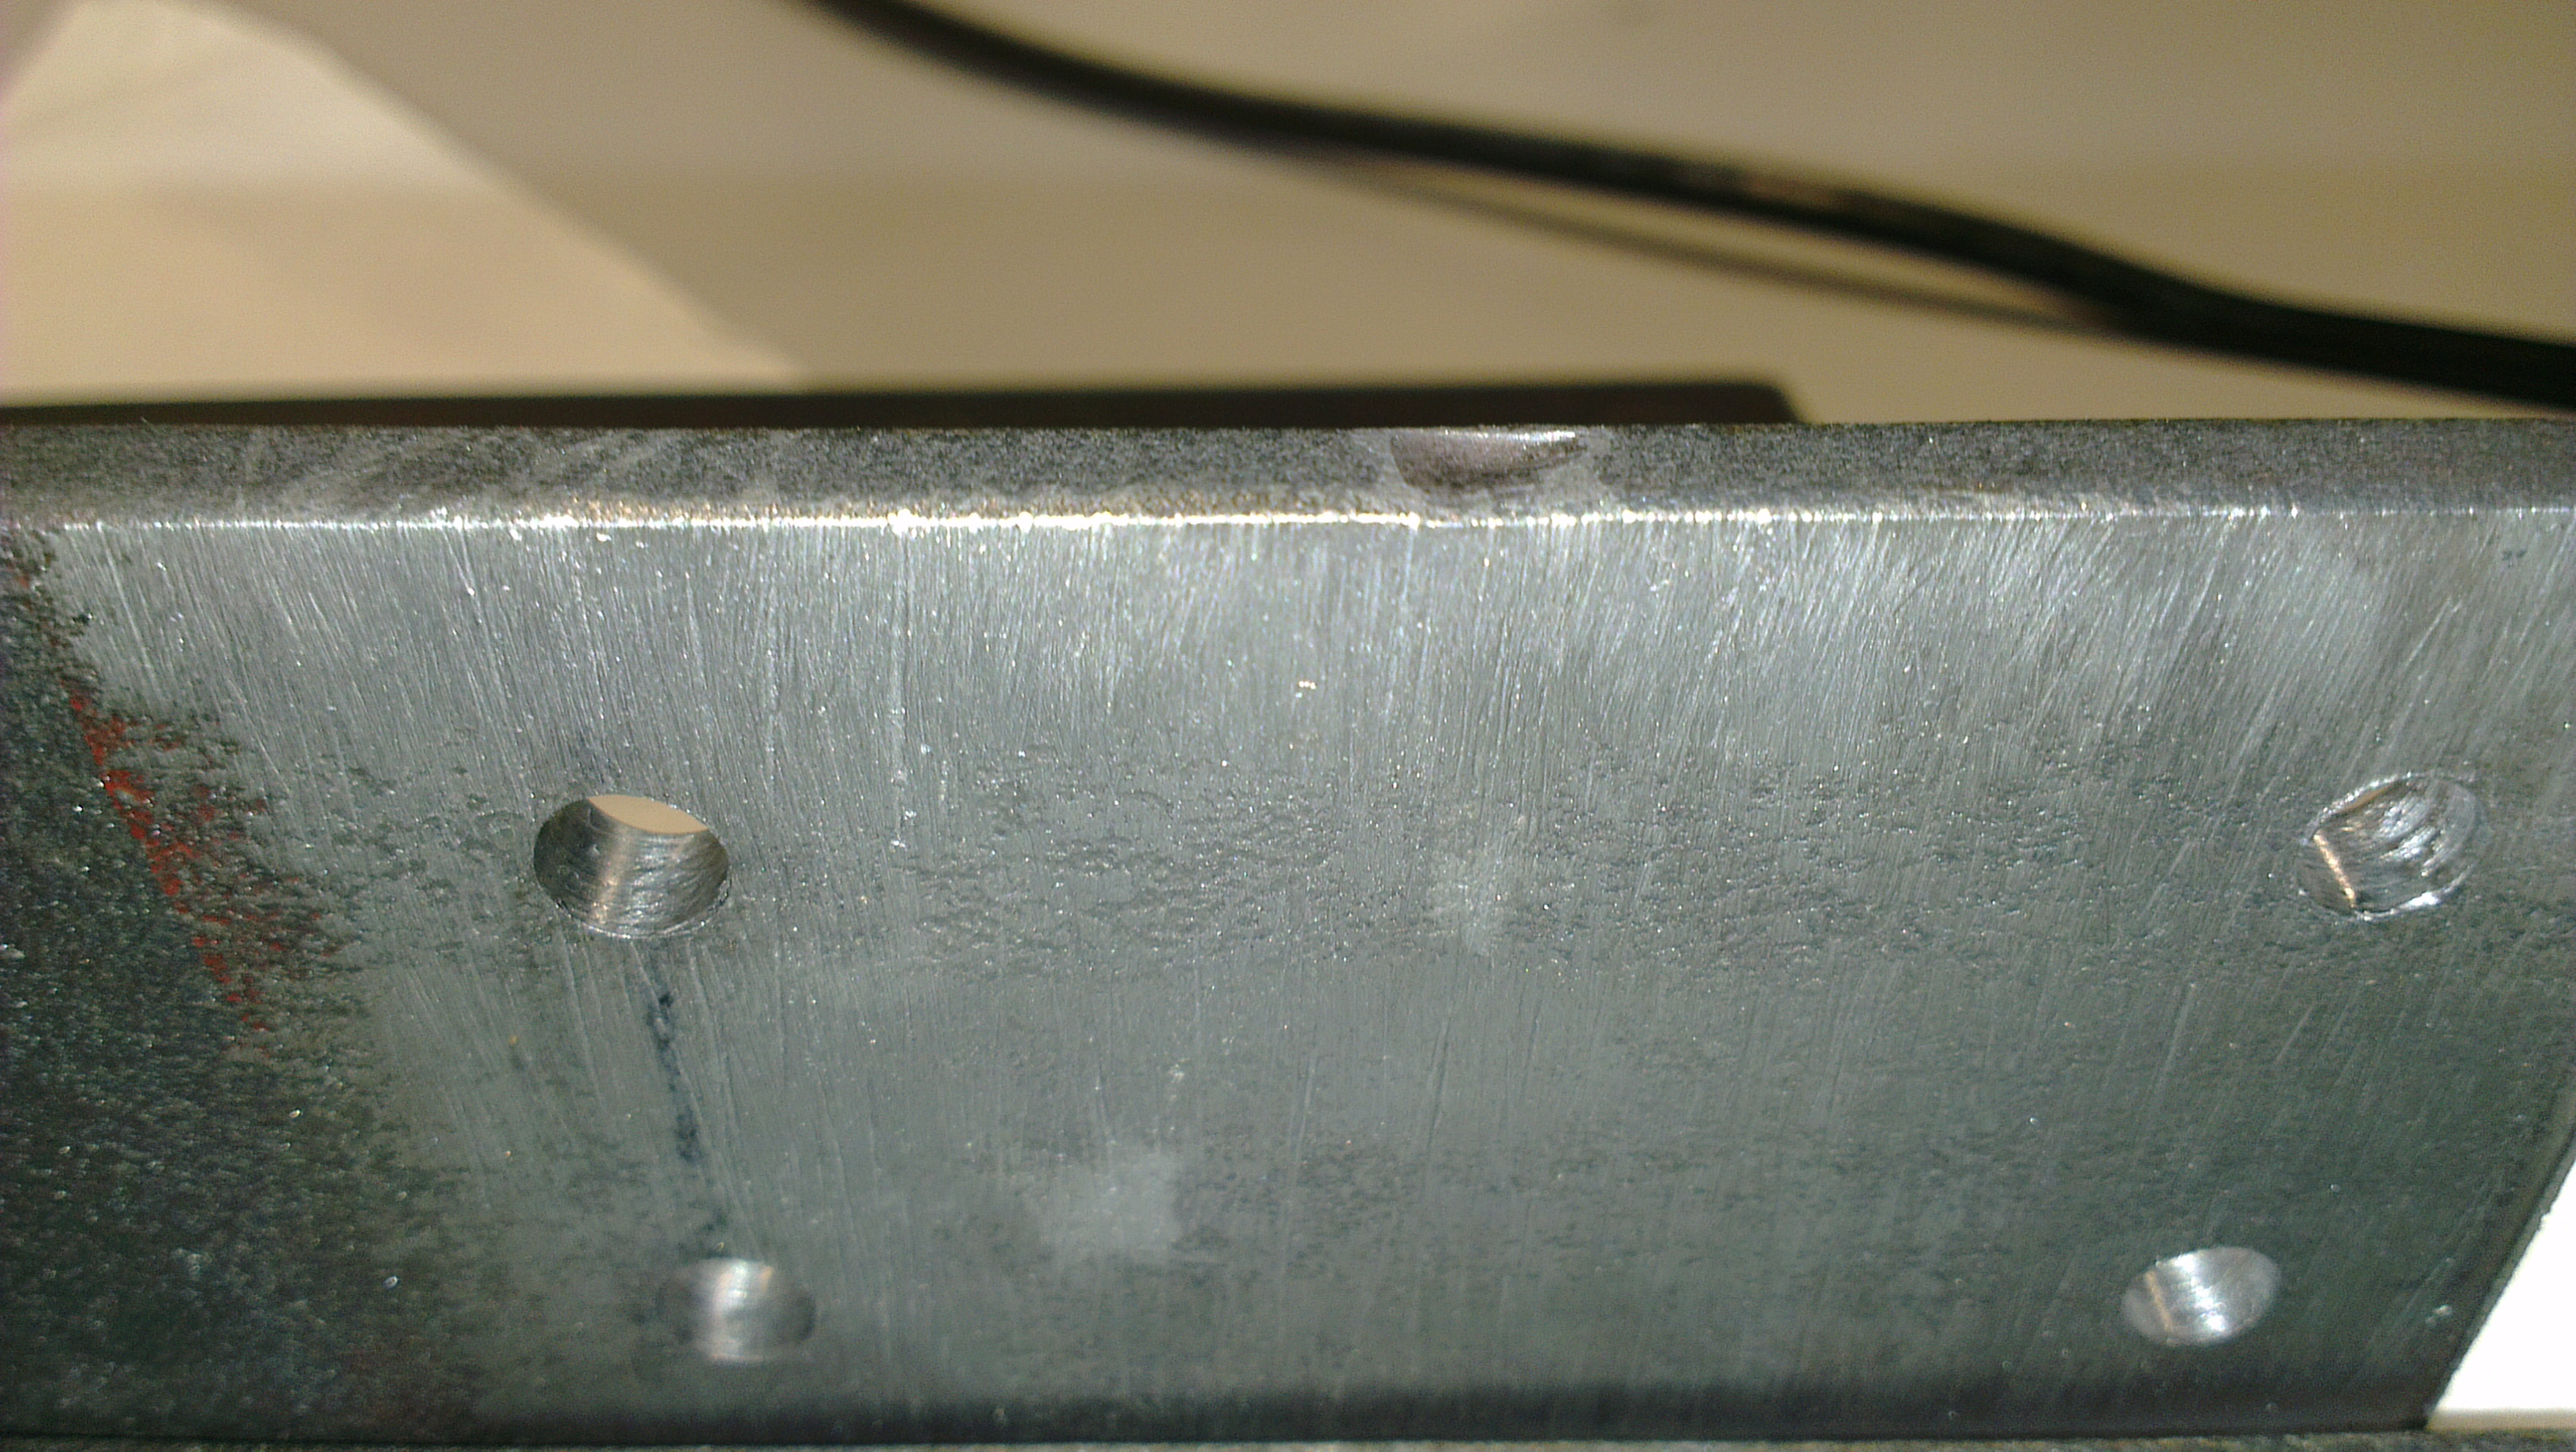
\includegraphics[width=\linewidth]{hak2}
  \caption{Hak sem myndaðist í einni stöng við prófun}
  \label{fig:hak2}
\end{figure}


\begin{figure}
  \centering
  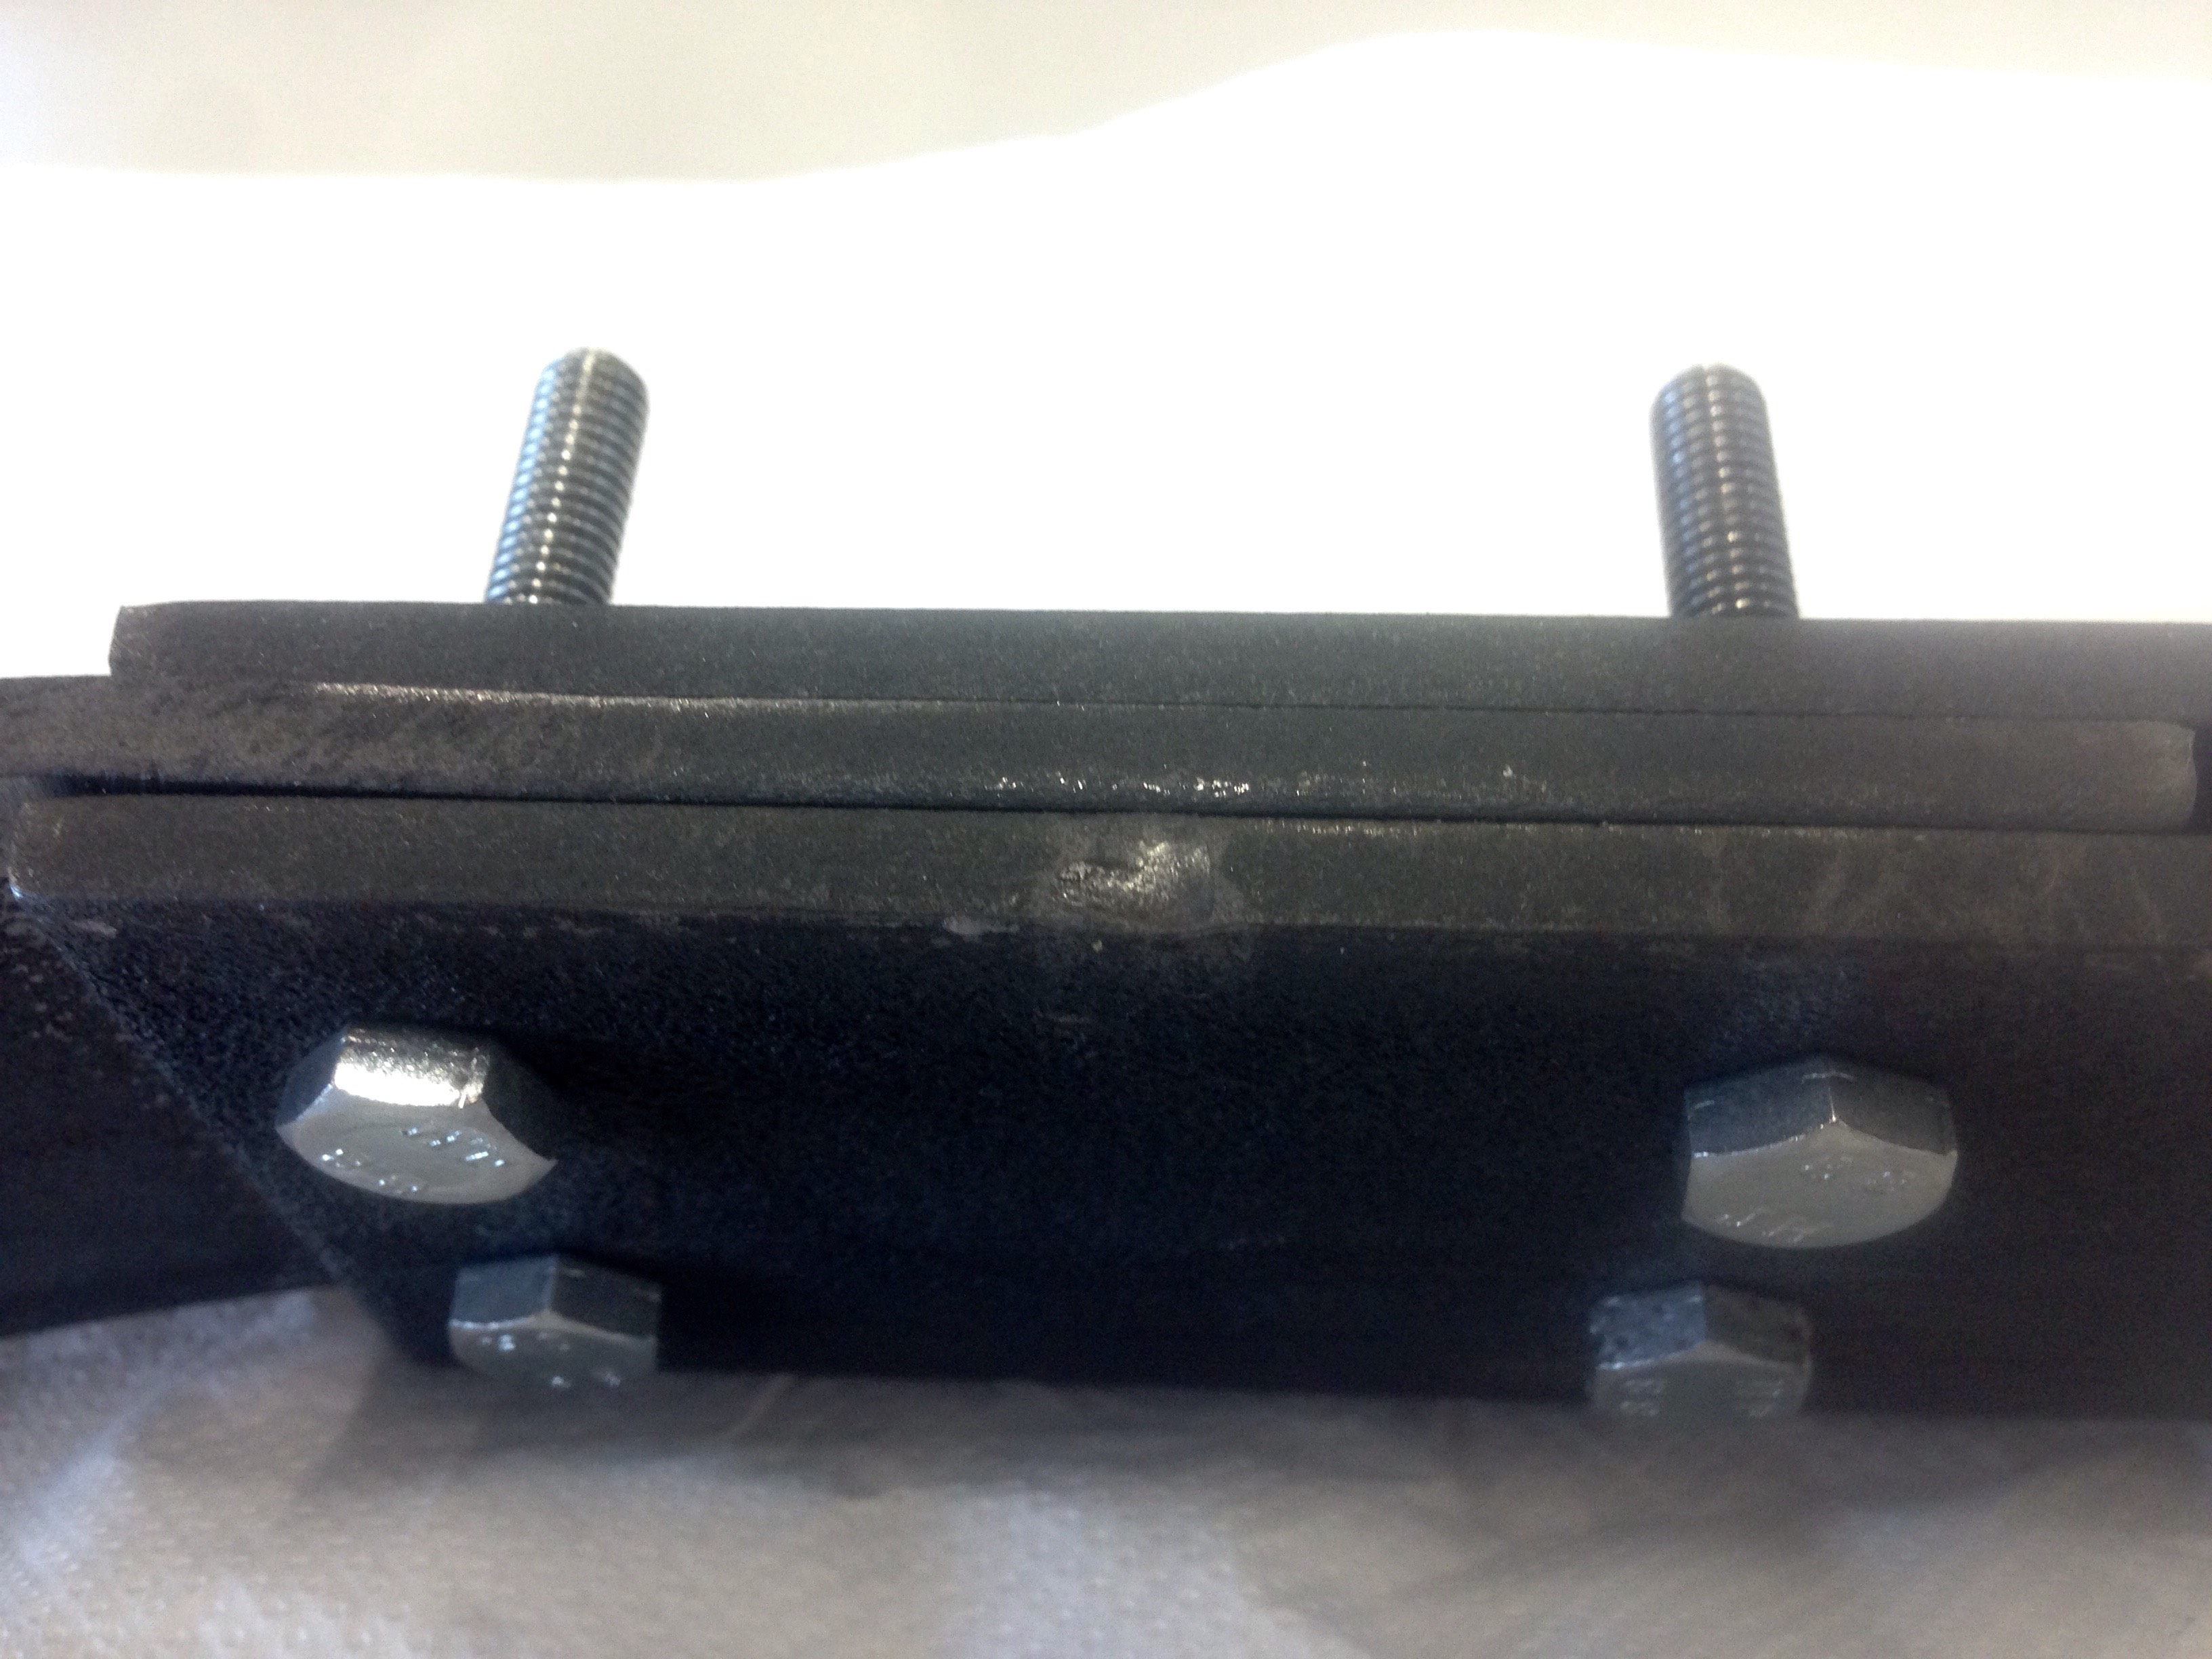
\includegraphics[width=\linewidth]{hak4}
  \caption{Hak sem myndaðist í einni stöng við prófun}
  \label{fig:hak4}
\end{figure}



Við álagsprófið beygluðust stálplöturnar en ekkert sá á boltunum, sbr. myndir \ref{fig:boltar}, \ref{fig:pano} og \ref{fig:exploded}.
Auk þess má sjá á stálplötunum að álagið var að mestu leyti á eina af ytri plötunum, sbr. myndir \ref{fig:hak}, \ref{fig:hak2} og \ref{fig:hak4}, og því var átakið skakkt. Þetta olli því að meira af álaginu fór í stálplöturnar, en minna af álaginu í boltana.
Það olli því að plöturnar beygluðust áður en nægt átak færi í boltana til að valda einhverju teljanlegu átaki á boltana.

\clearpage

\begin{figure}
  \centering
  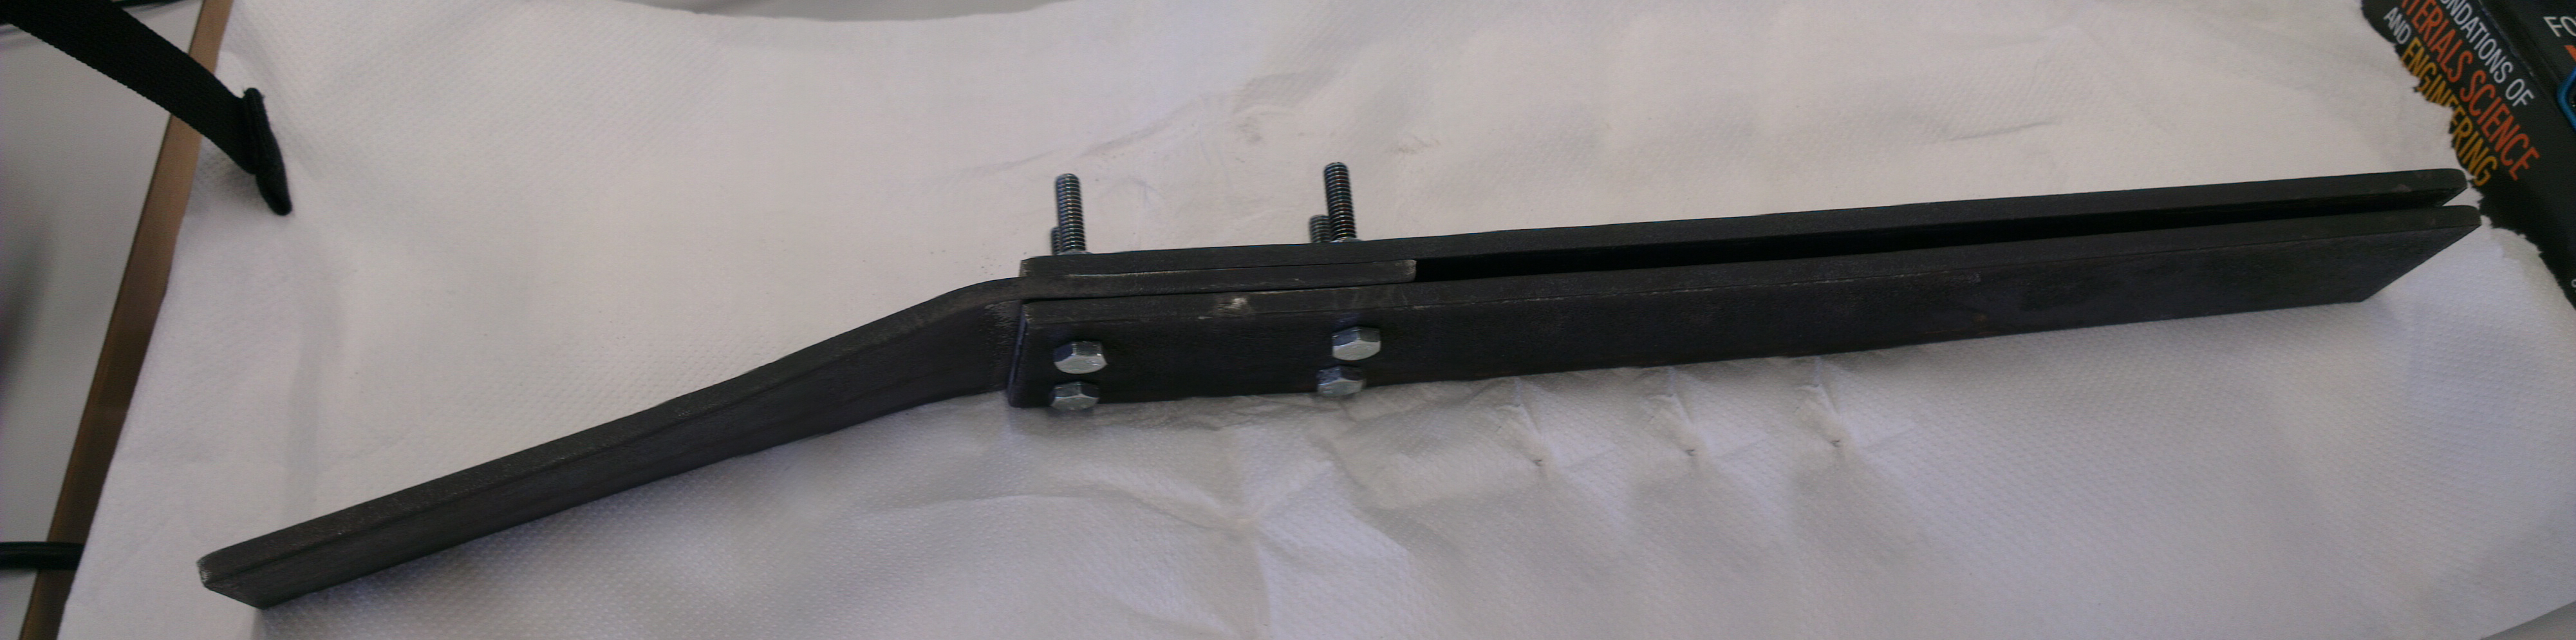
\includegraphics[width=\linewidth]{beygja_pano}
  \caption{Samsetning eftir prófun}
  \label{fig:pano}
\end{figure}


\begin{figure}
  \centering
  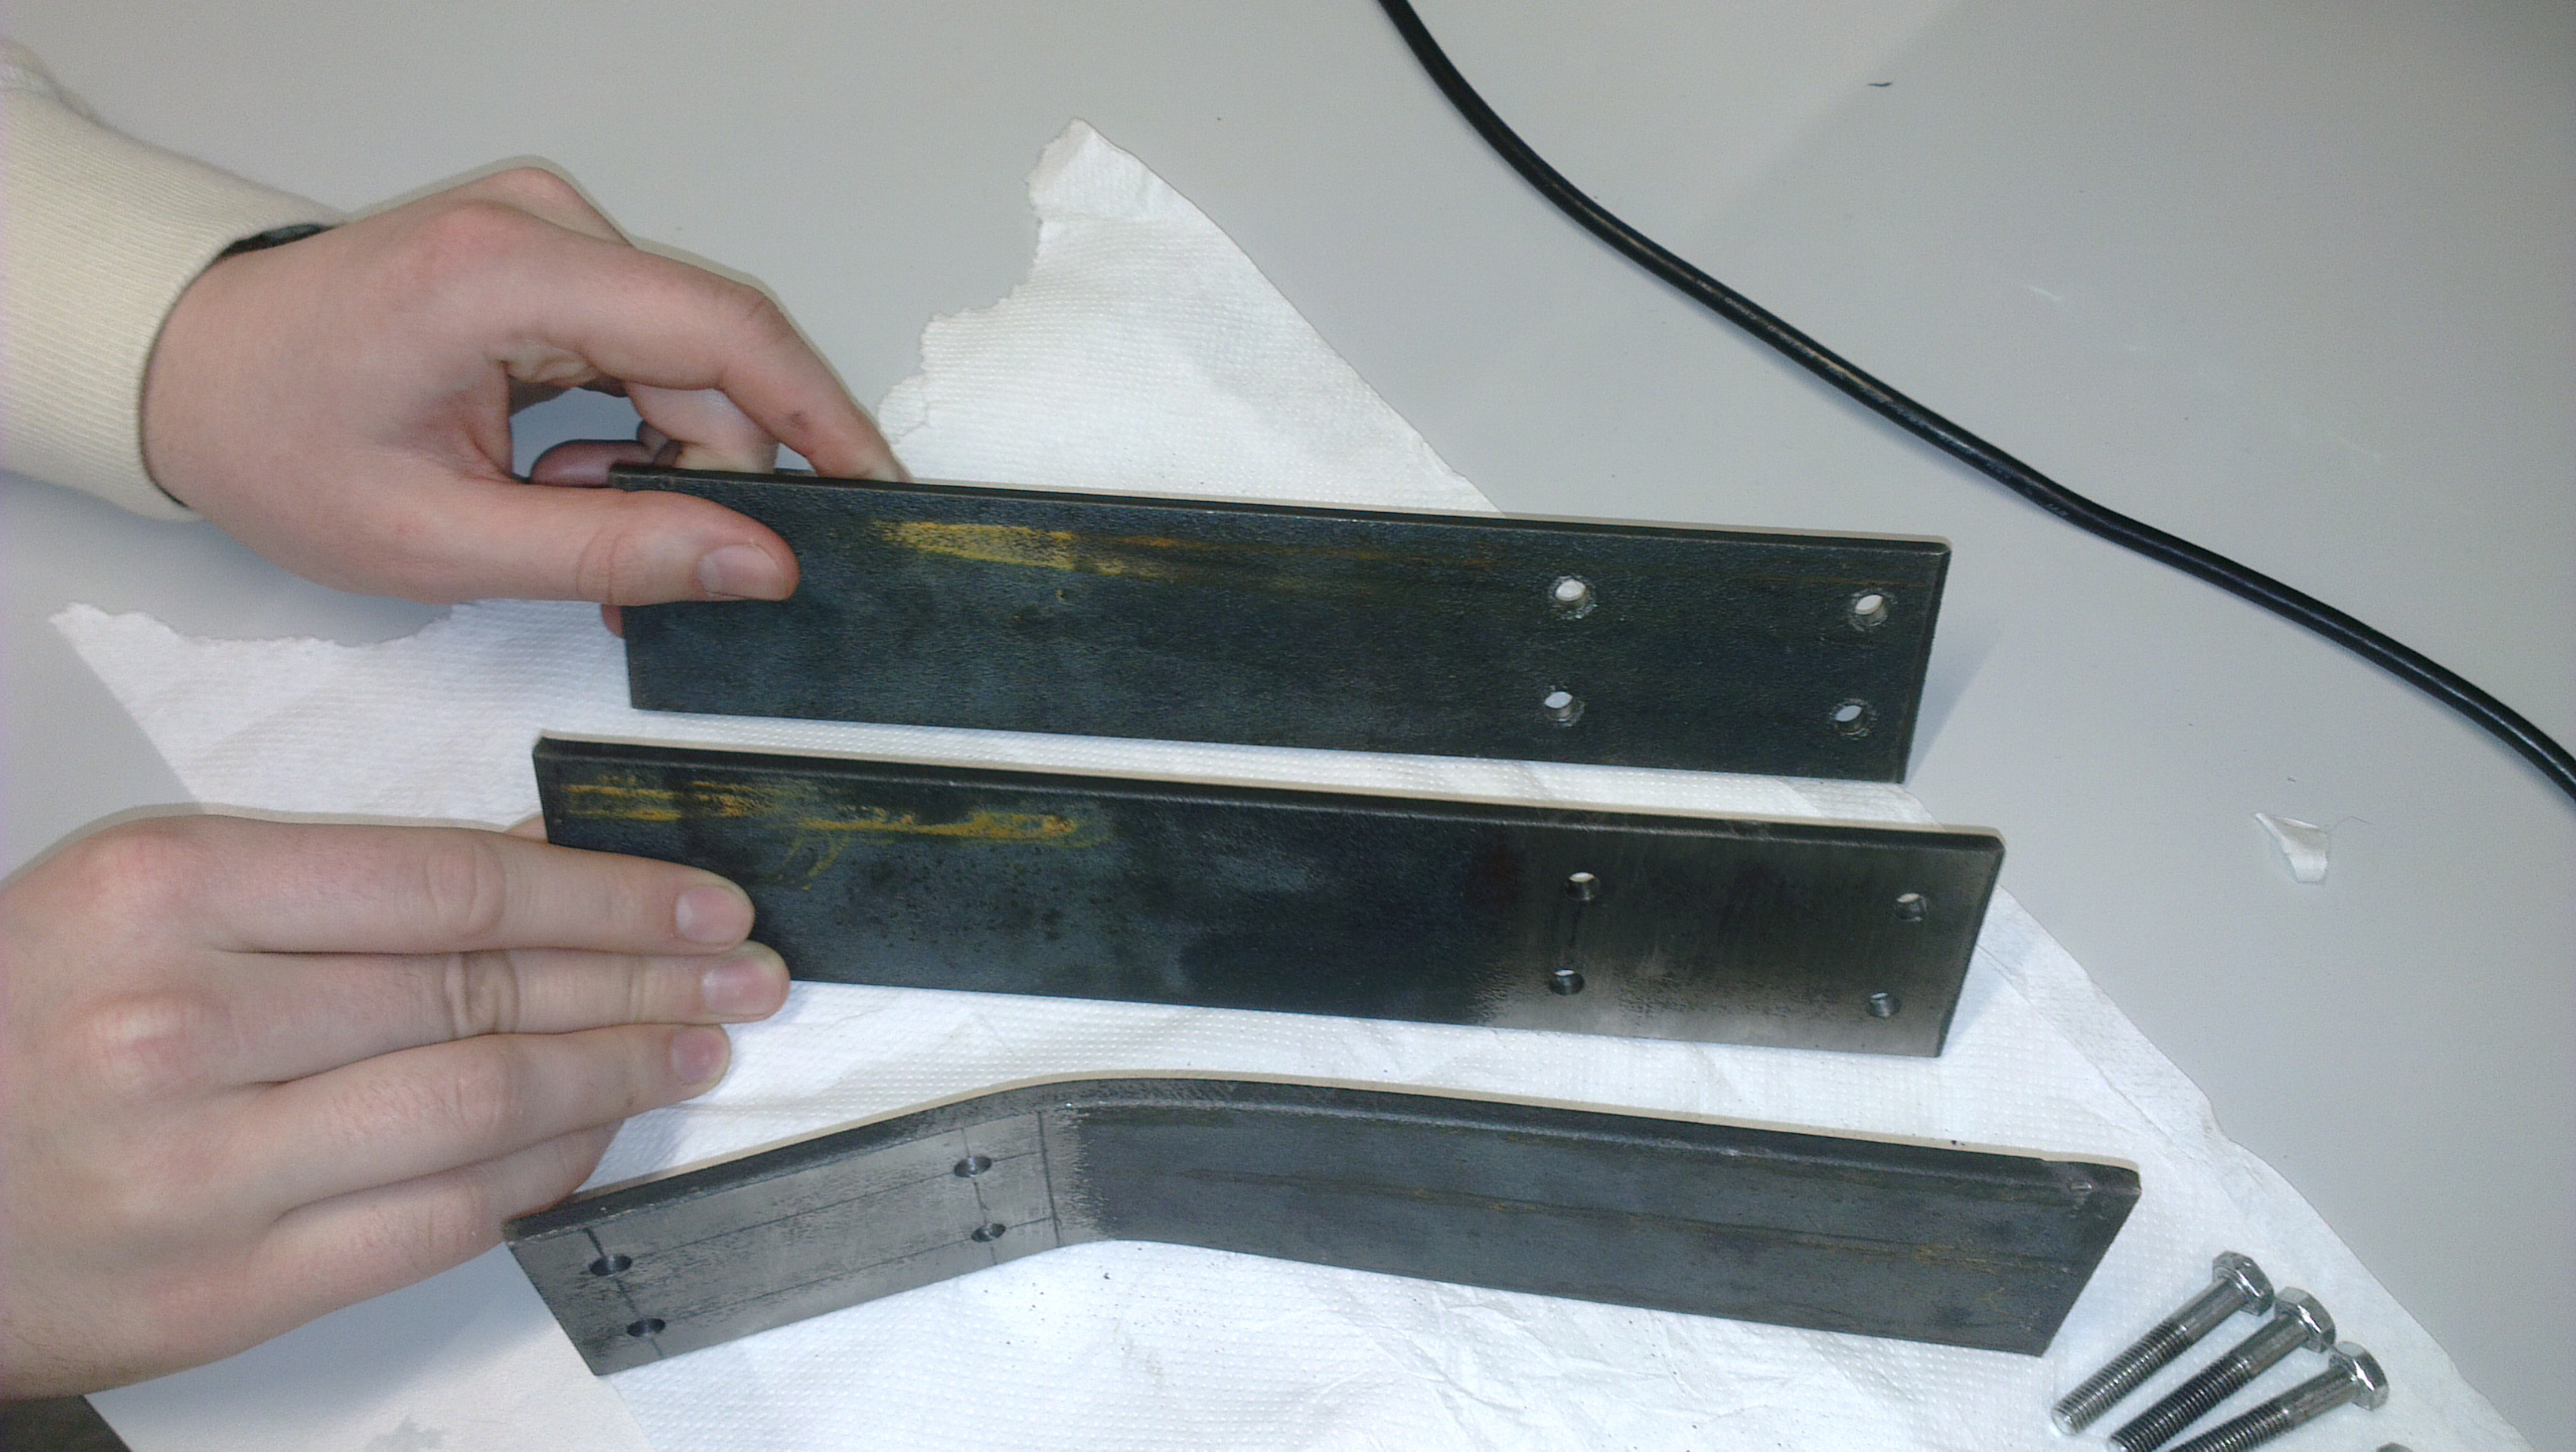
\includegraphics[width=\linewidth]{exploded_view}
  \caption{Tekið sundur eftir prófun}
  \label{fig:exploded}
\end{figure}

Því má í rauninni segja að prófið hafi verið gallað þar sem tækin voru ekki nógu nákvæm til að setja álagið beint í boltana. Það olli því að plöturnar gáfu ekki eftir eins og við gerðum ráð fyrir.

\printbibliography

\end{document}\\